\chapter{Conversion} 
\section{Conversion using the webservice}
While it is preferable to work in {\latex} from the start, this is not always possible. For edited volumes, for instance, it is common that not all authors can acquire the necessary skills in due course. For those cases, you can use the templates for MS Word and LibreOffice provided on \url{http://langsci-press.org/templatesAndTools}. Follow the instructions in the templates. When you are finished, upload your file to \url{http://glottotopia.org/doc2tex/doc2tex}. This will give you a file which you can copy into the skeleton (\figref{fig:conversion:glottotopia}). You have the choice between ``raw'' and ``mod''. Generally,  ``mod'' is preferable as a number of adaptations for linguists and \lsp are already in place. If you run into problems with ``mod'', you can use  ``raw'' as a fallback. You can then either copy and paste the converted document to a file of your own, or you can open the document directly in Overleaf (\figref{fig:conversion:overleaf}).

Note that the converter was built in 2015. Newer versions of MS Word/LibreOffice may introduce items unknown to the converter. In this case, contact support immediately.

\begin{figure}
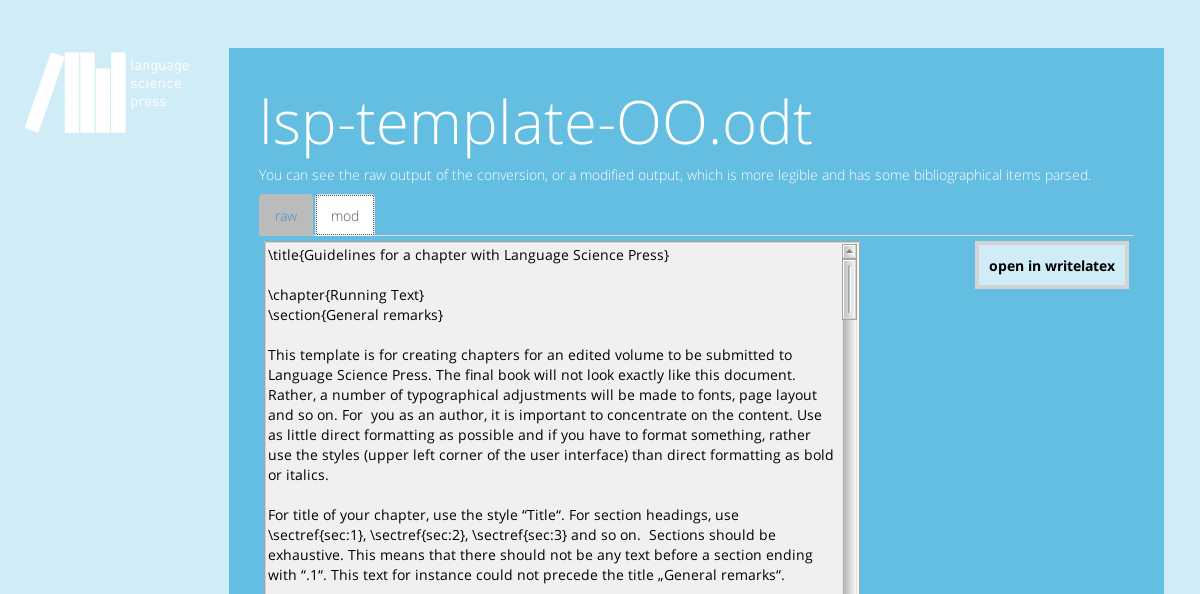
\includegraphics[width=\textwidth]{converter.png} 
\caption{After converting the template on \url{http://glottotopia.org/doc2tex/doc2tex}.}
\label{fig:conversion:glottotopia}
\end{figure}

\begin{figure}
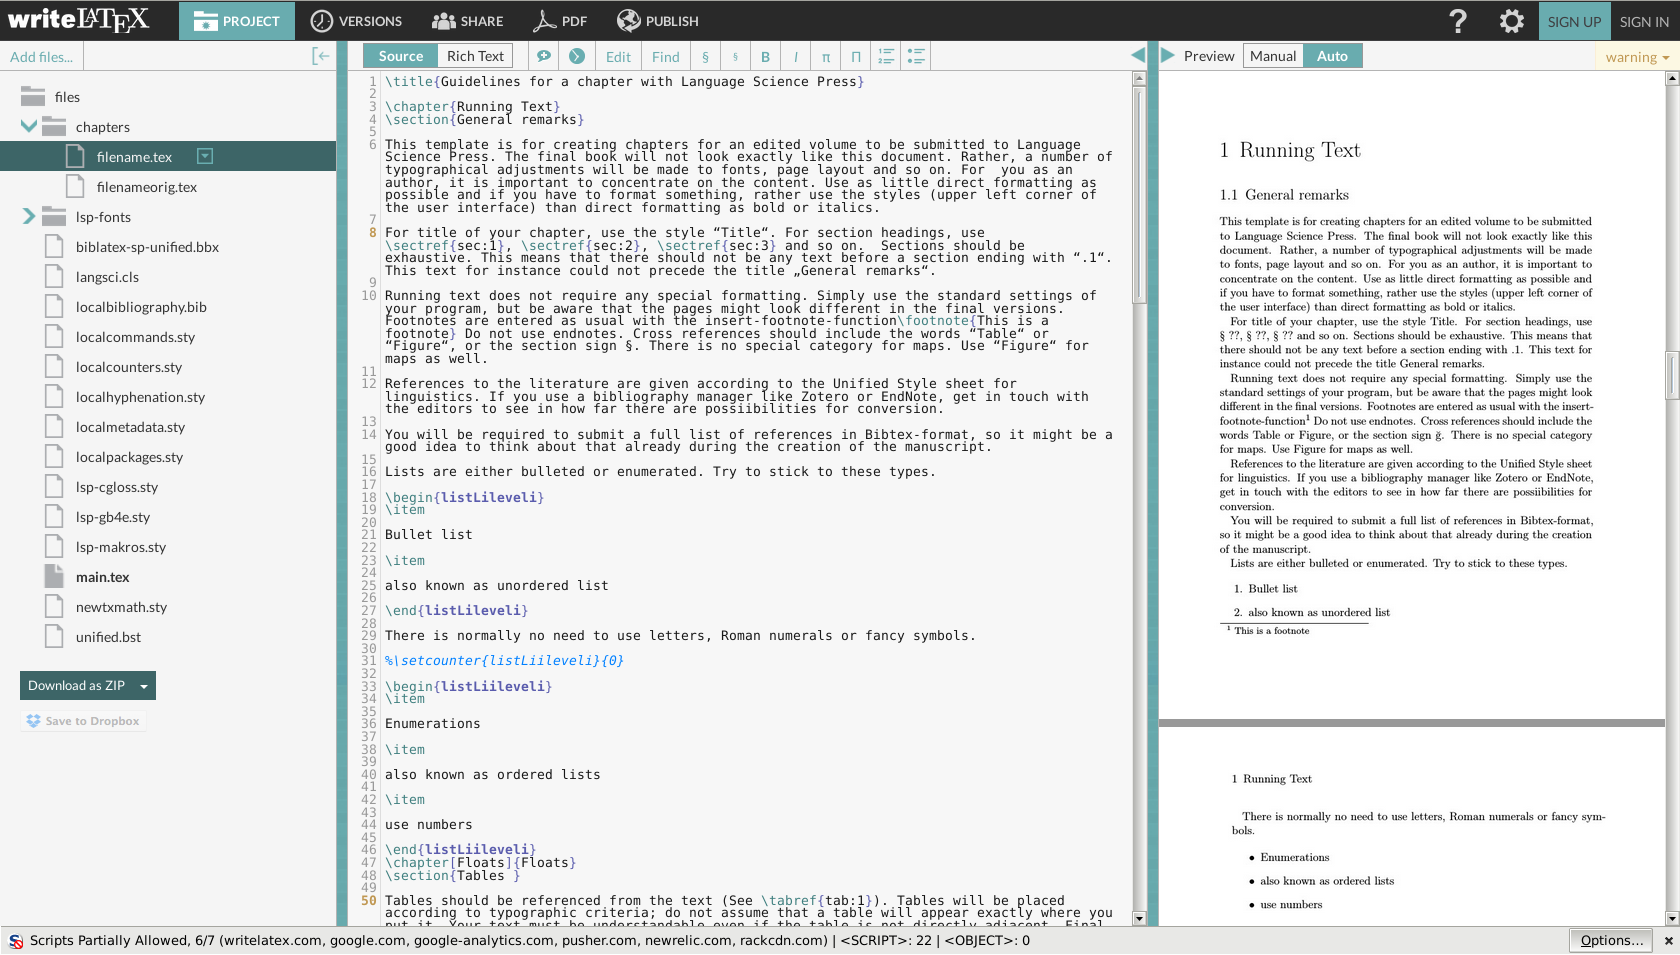
\includegraphics[width=\textwidth]{conversionwritelatex.png} 
\caption{Opening the converted document on Overleaf.}
\label{fig:conversion:overleaf}
\end{figure}

\section{Manual conversion}
If you want to convert your file on your local computer, you can use the program \verb+writer2latex+. The relevant command is 
\begin{verbatim}
w2l -wrap_lines_after=0 -multilingual=false 
-simple_table_limit=10 -use_supertabular=false 
-float_tables=true -float_figures=true 
-use_caption=true -image_options=width=\textwidth 
-inputencoding=utf8 -use_tipa=false -use_bibtex=true  
-formatting=convert_most -ignore_empty_paragraphs=true 
-use_color=false -page_formatting=ignore_all
 -use_hyperref=true mydocument.odt
\end{verbatim}

\section{Manual postprocessing}
While the converter tries to convert as much as possible, there are a some places where manual postprocessing is still required.
These include graphics, cross-references and some bibliographical references.

% \subsection{Examples}
% The output of automatically converted examples has the example formatting separated from the example content.  
% \begin{verbatim}
% \ea%1
%   \label{ex:1}
%   \langinfo{lg}{fam}{src}\\
%   \gll\\
%       \\
%   \glt
% \z
% 
% Ceci n' est pas une pomme
% 
%  this \textsc{neg}  {\cop.3\sg.\prs} \textsc{neg}   
% \textsc{det.f} apple
% 
% ``This is not an apple''
% \end{verbatim}
% 
% One has to manually join the former and the latter part to get
% 
% \begin{verbatim}
% \ea%1
%   \label{ex:1}
%     \langinfo{lg}{fam}{src}\\
%   \gll Ceci n'             est                 pas une pomme \\
%       this \textsc{neg} {\cop.3\sg.\prs} \textsc{neg}   
%       \textsc{det.f} apple\\
%   \glt ``This is not an apple''
% \z 
% \end{verbatim} 
% 
% Furthermore, \verb+\langinfo+ has to be adapted to reflect the correct language, family and source of the example, or removed altogether. In this case, one would use  \verb+\langinfo{French}{Indo-European}{René Magritte}\\+

\subsection{Graphics}
All graphics are commented out by default since the files will not be available on Overleaf until you upload them. So the following stretch

\begin{verbatim}
 \begin{figure}[h]
[Warning: Image ignored] %Unhandled or unsupported graphics:
%\includegraphics[width=\textwidth]
{a8dc5773011814b3b98013db7af4ec7e9-img1.png}
\caption[Some caption]{Some caption}
\end{figure}
\end{verbatim}

has to become


\begin{verbatim}
\begin{figure}
 \includegraphics[width=\textwidth]{figures/realnameofthefile.png}
 \caption{Some caption}
 \label{fig:chaptername:filehandle}
\end{figure}
\end{verbatim}

\subsection{Cross-references}
Generally, references to sections and examples should work. Occasionally, there might be problems with stretches like ``(12a)'' or ``(12-15)''. These have to be fixed manually.

\subsection{Bibliographical references}
The most common bibliographical references should work. Where authors have names which consist of two parts (such as ``Van Valin''), the author is often misrecognized as ``Valin''. Also, stretches like ``Smith 2000, 2001a,b, 2002'' will need manual postprocessing. 




